%%%%%%%%%%%%%%%%%%%%%%%%%%%%%%%%%%%%%%%%%%%%%%%%%%%%%%%%%%%%%%%%%%%%%%%%%%%%%%%%
%%
%%   BornAgain User Manual
%%
%%   homepage:   http://www.bornagainproject.org
%%
%%   copyright:  Forschungszentrum Jülich GmbH 2015
%%
%%   license:    Creative Commons CC-BY-SA
%%   
%%   authors:    Scientific Computing Group at MLZ Garching
%%               C. Durniak, M. Ganeva, G. Pospelov, W. Van Herck, J. Wuttke
%%
%%%%%%%%%%%%%%%%%%%%%%%%%%%%%%%%%%%%%%%%%%%%%%%%%%%%%%%%%%%%%%%%%%%%%%%%%%%%%%%%


\newpage
\chapter{Online documentation}
  \label{sec:online}

This User Manual is complementary to the online documentation
at the project web site \url{http://www.bornagainproject.org}.
It does not duplicate information that is more conveniently
read online.
This brief chapter contains no more than a few pointers to the web site.

\begin{figure}[ht]
\begin{center}
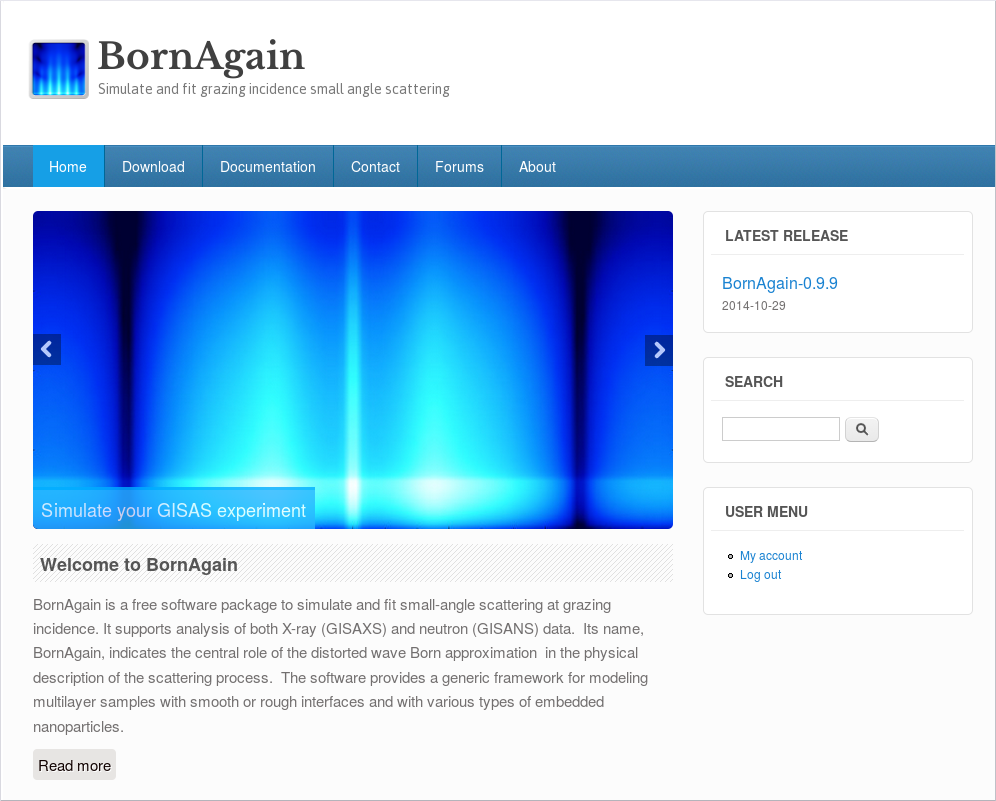
\includegraphics[width=0.83\textwidth]{fig/screenshot/website.png}
\end{center}
\caption{A screenshot of the home page
         \url{http://www.bornagainproject.org}.}
\label{fig:website}
\end{figure}


%%%%%%%%%%%%%%%%%%%%%%%%%%%%%%%%%%%%%%%%%%%%%%%%%%%%%%%%%%%%%%%%%%%%%%%%%%%%%%%%
\section{Download and installation}
%%%%%%%%%%%%%%%%%%%%%%%%%%%%%%%%%%%%%%%%%%%%%%%%%%%%%%%%%%%%%%%%%%%%%%%%%%%%%%%%
  \index{Download}%
  \index{Installation}%

\BornAgain\
\index{Platform (operating system)}%
\index{Operating system}%
is a multi-platform software.
We actively support the operating systems
Linux,
\index{Linux}%
MacOS
\index{MacOS}%
and  Microsoft Windows.
\index{Windows|see {Microsoft Windows}}%
\index{Microsoft Windows}%
The \textsc{Download} section on the \BornAgain\ web site
points to the download location for
binary and source packages.
It also provides a link to our \Code{git} server
where the unstable development trunk is available
for contributors or for users who want to live on the edge.

The \textsc{Documentation} section contains
pages with \textit{Installation instructions}.


%%%%%%%%%%%%%%%%%%%%%%%%%%%%%%%%%%%%%%%%%%%%%%%%%%%%%%%%%%%%%%%%%%%%%%%%%%%%%%%%
\section{Further online information}
%%%%%%%%%%%%%%%%%%%%%%%%%%%%%%%%%%%%%%%%%%%%%%%%%%%%%%%%%%%%%%%%%%%%%%%%%%%%%%%%

The \textsc{Documentation} section of the project web site
contains in particular
\begin{itemize}
\item an overview of the software architecture,
\item a list of implemented functionality,
\item tutorials for ``Working with \BornAgain'',
      using either the Graphical User Interface or
      \Python\ scripts,
         \index{Tutorials}
\item a comprehensive collection of tutorial examples that demonstrate
   how to use \BornAgain\ for modeling various sample structures
    and different experimental conditions,
\item a link to the API reference for using \BornAgain\ through
   \Python\ scripts or C$++$ programs.
\index{API|see {Application programming interface}}%
\index{Application programming interface}%
\index{Python}%
\index{C++@C$++$}
\end{itemize}


%%%%%%%%%%%%%%%%%%%%%%%%%%%%%%%%%%%%%%%%%%%%%%%%%%%%%%%%%%%%%%%%%%%%%%%%%%%%%%%%
\section{Registration, contact, discussion forum}\label{Snews}
%%%%%%%%%%%%%%%%%%%%%%%%%%%%%%%%%%%%%%%%%%%%%%%%%%%%%%%%%%%%%%%%%%%%%%%%%%%%%%%%

\index{Registration}
\index{Newsletter}
To stay informed about the ongoing development of \BornAgain,
register on the project homepage \url{http://www.bornagainproject.org}
(``Create new account'').
You will then receive our occasional newsletters,
and be authorized to post to the discussion forum.

To contact the \BornAgain\ development and maintenance team
in the Scientific Computing Group
of Heinz Maier-Leibnitz Zentrum (MLZ) Garching,
write a mail to \url{contact@bornagainproject.org},
or fill the form in the \textsc{Contact} section of the
project web site.

\index{Forum}
For questions that might be of wider interest,
please consider posting to the discussion forum,
accessible through the \textsc{Forums} tab of the project web site.
